\chapter{Quelques pistes\\pour préparer la\\leçon au concours} \label{Tra0}

\bigskip

\begin{figure}[h]
   \centering
      
\includegraphics[height=6cm]{Transversal/Images/Tra0_cours_prof}
\end{figure}

\begin{prerequis}[Un peu d'histoire]
   Les écoles normales, depuis le début du 19\up{e} siècle, puis les IUFM en 1989, les ESPE en 2013 et enfin (pour l'instant !) les INSPE en 2019 sont des établissements chargés de former les instituteurs, puis les professeurs des écoles, de collège et lycée et de lycées professionnels. \\
   À partir de 1990, le corps des professeurs des écoles nait et le CRPE comprend 2 épreuves d'admissibilité (français, maths), ainsi que quatre épreuves d'admission (oral pro, option, EPS et entretien). Le concours se passait à la fin de la première année et le stage en deuxième année, en alternance. \\
   En 2005, le concours est composé de trois épreuves d'admissibilité écrites (français, maths, GH et sciences) et trois entretiens oraux (EPS, LVE, oral pro). \\
   En 2010, une réforme voit le jour, et les candidats sont dans l'obligation d'être titulaire d'un master 2 pour devenir professeur des écoles. Le concours, quant à lui, reste le même. \\
   En 2015, une nouvelle réforme a lieu, les épreuves d'admissibilité sont réduites à deux matières (français et maths), et deux épreuves d'admission orales (dossier et connaissance du système éducatif, puis EPS). \\
   À partir de 2022, après une énième réforme, l'admissibilité repasse à trois épreuves (français, maths et arts-HGEMC-sciences au choix) et deux épreuves orales (leçon en français-maths et entretien), en plus d'une épreuve facultative de langues. 
\end{prerequis}


%%%%%%%%%%%%%%%%%%%%%%%%%%%%%%
%%%%%%%%%%%%%%%%%%%%%%%%%%%%%%
\cours


%%%%%%%%%%%%%%%%%%%%%%%%%%%%%%%
\section{Les épreuves au concours à partir de la session 2022} 

Et comme une infographie vaux mieux qu'un long discours\dots
\begin{center}
   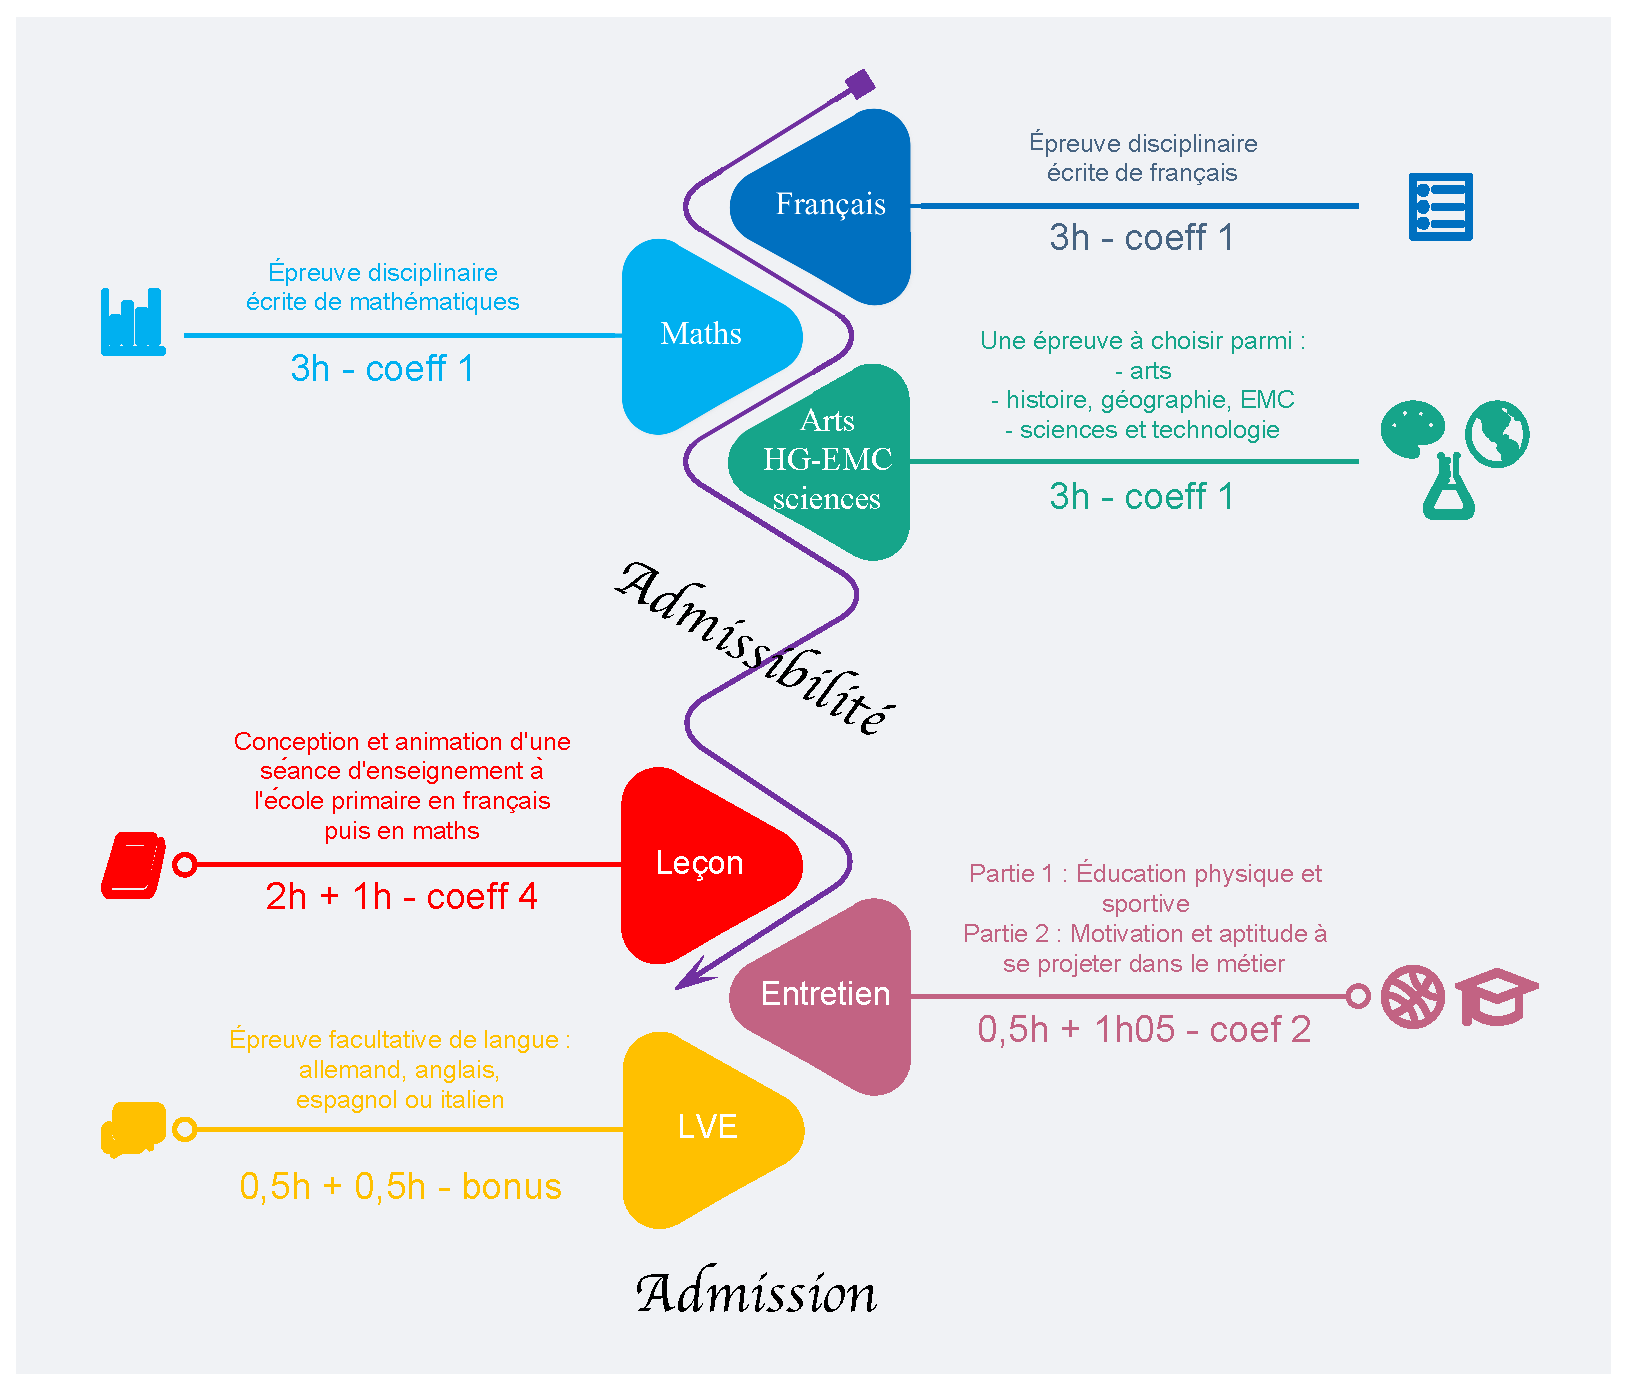
\includegraphics[width=17cm]{Transversal/Images/Tra0_cours_infographie}
\end{center}

Concernant l'{\bf épreuve écrite de mathématiques}, d'une durée de 3h, elle est constituée d'un ensemble d'au moins trois exercices indépendants (pour la session 2022, les différents sujets étaient composés de quatre ou cinq exercices), permettant de vérifier les connaissances disciplinaires. Elle est notée sur 20 et une note inférieure ou égale à 5 est éliminatoire, tout comme les autres épreuves écrites. \\

L'{\bf épreuve de leçon} est d'une durée de 1h de préparation commune (français et maths), suivie de deux parties de 30 minutes chacune en français et en maths (10 à 15 minutes d'exposé et le reste d'entretien avec le jury). Le sujet comporte deux dossiers (français et maths). Chacun est constitué d'au plus quatre documents de nature variée : supports pédagogiques, extraits de manuels scolaires, traces écrites d'élèves, extraits des programmes\dots{} et le candidat doit concevoir et animer une séance d'enseignement sur le thème donné.

\bigskip


%%%%%%%%%%%%%%%%%%%%%%%%%%%
\section{Les repères institutionnels en mathématiques} 

\smallskip
Sur éDUSCOL, on trouve moult ressources officielles pour préparer sa classe dans les différentes disciplines. Concernant les mathématiques, on peut télécharger les ressources suivantes (liens cliquables). \medskip

Pour le \uline{cycle 1} [édu1], il est possible de consulter le \href{https://eduscol.education.fr/document/20062/download}{\blue programme consolidé} publié au BO du 24 juin 2021, ainsi que des {\bf ressources d'accompagnement} dans les domaines 4 (\href{https://eduscol.education.fr/2819/acquerir-les-premiers-outils-mathematiques}{\blue Acquérir les premiers outils mathématiques}) et 5 (\href{https://eduscol.education.fr/2822/se-reperer-dans-le-temps-et-l-espace}{\blue Se repérer dans le temps et dans l'espace}). \medskip

Pour les \uline{cycles 2 et 3} [édu2] [édu3], on dispose de plusieurs types de ressources. \\
$\bullet$ Les {\bf programmes de cycle} présentent les enjeux et les objectifs de formation de chaque cycle et mettent en évidence la contribution des différents champs disciplinaires à l'acquisition de chacun des cinq domaines de formation du socle commun. \\
$\bullet$ Les {\bf repères annuels de progression} offrent une référence commune et doivent permettre d'aborder de façon équilibrée les connaissances et compétences tout au long des trois années de chaque cycle. \\
$\bullet$ Les {\bf attendus de fin d'année} fixent un horizon en termes de connaissances et de compétences pour chaque niveau. Des exemples de réussite sont proposés afin d'illustrer ce que doit savoir faire l'élève de la fin du CP à la fin de la classe de 3\up{e}. \\
Outre ces trois types de ressources incontournables pour la préparation de progressions et de programmations, on y trouve également des {\bf ressources thématiques} qui sont des pistes et des stratégies d'enseignement concrètes sur des notions des différents thèmes ainsi que des {\bf ressources d'évaluation} proposant une aide à l'évaluation du niveau de maîtrise des domaines du socle commun en fin de cycle. \medskip

Tableau récapitulatif des ressources institutionnelles principales en élémentaire. \smallskip

\begin{center}
   {\hautab{1.5}
   \begin{ltableau}{0.85\linewidth}{2}
      \hline
      Cycle 2 & Cycle 3 \\
      \hline
      \href{https://www.education.gouv.fr/media/70279/download}{\blue Programme du cycle 2 (juin 2020)}
      &
      \href{https://www.education.gouv.fr/media/70282/download}{\blue Programme du cycle 3 (juin 2020)}
      \\
      \multicolumn{2}{|c|}{\href{https://eduscol.education.fr/137/attendus-de-fin-d-annee-et-reperes-annuels-de-progression-du-cp-la-3e}{\blue Attendus de fin d'année et repères annuels de progression du CP au CM2}}
      \\
      \hline
      \href{https://eduscol.education.fr/document/3738/download?attachment}{\blue Pour enseigner les nombres, le calcul} \newline
      \href{https://eduscol.education.fr/document/3738/download?attachment}{\blue et la résolution de problèmes au CP}
      &
      \href{https://eduscol.education.fr/document/32206/download?attachment}{\blue La résolution de problèmes mathématiques} \newline
      \href{https://eduscol.education.fr/document/32206/download?attachment}{\blue au cours moyen}
      \\
      \multicolumn{2}{|c|}{\href{https://eduscol.education.fr/document/15400/download}{\blue Le calcul aux cycles 2 et 3}}
      \\
      \href{https://eduscol.education.fr/document/15403/download}{\blue Le calcul en ligne au cycle 2}
      &
      \href{https://eduscol.education.fr/document/16507/download}{\blue Le calcul en ligne au cycle3}
      \\
      &
      \href{https://eduscol.education.fr/document/16510/download}{\blue Fractions et nombres décimaux au cycle 3}
      \\
      \hline
      \href{https://eduscol.education.fr/document/15406/download}{\blue Grandeurs et mesures au cycle 2}
      &
      \href{https://eduscol.education.fr/document/16513/download}{\blue Grandeurs et mesures au cycle 3}
      \\
      \hline
      &
      \href{https://eduscol.education.fr/document/16516/download}{\blue Espace et géométrie au cycle 3} \\
      \multicolumn{2}{|c|}{\href{https://eduscol.education.fr/document/15409/download}{\blue Initiation à la programmation aux cycle 2 et 3}}
      \\
      \hline
      &
      \href{https://eduscol.education.fr/document/16522/download}{\blue Résoudre des problèmes de} \newline
      \href{https://eduscol.education.fr/document/16522/download}{\blue proportionnalité au cycle 3}
      \\
      \hline
   \end{ltableau}}
\end{center}

\bigskip


%%%%%%%%%%%%%%%%%%%%%%%%%%%
\section{Construction d'une séquence, d'une séance}

\subsection{Progression, programmation} %%%

Avant de commencer à préparer ses séances, il est nécessaire d'avoir tout d'abord réfléchi à la progression et la programmation des apprentissages.

\begin{center}
   \begin{minipage}{6cm}
      \begin{ltableau}{\linewidth}{1}
         \hline
         {\bf Progression} \\
         \hline
         Vient de \og progrès \fg \\
         Elle établit un ordre dans les apprentissages par des étapes successives parmi les notions, tout en tenant compte des acquis des élèves. \\
         Facteur : les SAVOIRS \\
         \hline
      \end{ltableau}
   \end{minipage}
   \qquad
   \begin{minipage}{6cm}
      \begin{ltableau}{\linewidth}{1}
         \hline
         {\bf Programmation} \\
         \hline
         Vient de \og programme \fg \\
         Elle se préoccupe de la distribution chronologique des séquences dans le cadre de la progression et prend en compte le calendrier scolaire. \\
         Facteur : le TEMPS \\
         \hline
      \end{ltableau}
   \end{minipage}

\begin{pspicture}(0,0)(17,1)
   \psline{->}(5,1)(7,0.1)
   \psline{->}(12,1)(10,0.1)
\end{pspicture}

   \begin{ltableau}{0.65\linewidth}{1}
      \hline
      {\bf Séquence} \\
      \hline
      Ensemble de plusieurs séances liées entre elles par un même objectif. \\
      Unité de SENS \\ [1mm] 
      \begin{tabular}{|p{2cm}|p{2cm}|p{2cm}|p{2cm}|} 
         \hline
         \multicolumn{4}{|c|}{\cellcolor{FondTableaux}{\bf Séances}} \\
         \hline
         \multicolumn{4}{|c|}{Période d'enseignement d'une séquence.} \\
         \multicolumn{4}{|c|}{Unité de TEMPS}\\
         \hline
        Séance 1 & Séance 2 & \dots & Séance $n$ \\
         \hline
         \dots & \dots & & \dots \\ [8mm] 
         \hline
      \end{tabular} \\
      \\ [-3mm]
      \hline
   \end{ltableau}
\end{center}


\subsection{Séquence} %%%

Plus précisément, le BO stipule qu'une {\bf séquence d'enseignement }est définie comme \og un ensemble continu ou discontinu de séances, articulées entre elles dans le temps et organisées autour d'une ou plusieurs activités en vue d'atteindre des objectifs fixés par les programmes d'enseignement \fg. La séquence mène les élèves à un nouveau savoir ou savoir-faire qui prépare les acquisitions ultérieures. \medskip

Il existe plusieurs types de séances : \\
$\bullet$ {\bf La séance de découverte} : elle permet de susciter l'intérêt des élèves. Les élèves découvrent : manipulent, expérimentent, questionnent, se familiarisent avec le matériel considéré ou les notions abordées. \\
$\bullet$ {\bf La séance de structuration} : après la séance de découverte, les élèves savent quels savoirs sont mis en jeu, mais il leur manque des connaissances. Ils doivent passer de l’action à la formulation. C’est un bon moment pour comparer les résultats, réflexion, verbaliser\dots{} jusqu'à obtenir une trace écrite. \\
$\bullet$ {\bf La séance d'entraînement} : les élèves sont amenés à répéter ce qu'ils ont appris lors de la séance précédente pour s’approprier les solutions, les mémoriser.
Une fois qu’ils savent faire en réception, il faut également s’assurer qu’ils sont capables de produire une situation mettant en jeu cette compétence. \\
$\bullet$ {\bf La séance de réinvestissement} : l’élève réinvestit son savoir dans un autre contexte, un autre domaine que celui de l’apprentissage initial. Il va renforcer, consolider et fixer ses acquis en les généralisant (ouverture, élargissement).


\subsection{Construction d'une séance} %%%

La construction d'une séance est souvent matérialisée par une fiche de préparation. Celle-ci est assez personnelle et il en existe de plusieurs sortes. Toutefois, on y retrouve quelques invariants. Par exemple : \\

{\small\hautab{1.35}
\begin{tabular}{|p{8.1cm}|p{8.2cm}|}
   \hline
   \multicolumn{2}{|c|}{\cellcolor{FondTableaux}{\bf Titre de la séance}} \\
   \hline
   Enseignement : \textcolor{gray}{mathématiques} & {\footnotesize Nombres et calculs - Grandeurs et mesures - Espace et géométrie} \\
   Séquence : & Place de la séance dans la séquence : \\
   \hline
   \multicolumn{2}{|p{16.5cm}|}{Compétences travaillées/domaines du socle :} \\
   \multicolumn{2}{|p{16.5cm}|}{Attendus de fin de cycle :} \\
   \multicolumn{2}{|p{16.5cm}|}{Objectif(s) de l’activité : \textcolor{gray}{savoirs (connaissances) et/ou savoirs-faire (capacités). Il est formulé à l'aide d'un verbe d'action et il décrit le résultat attendu sans préciser la stratégie à mettre en œuvre pour l'atteindre.}} \\
   \multicolumn{2}{|p{16cm}|}{Prérequis : } \\
   \hline
   Cycle : & Niveau de classe : \\
   Période de l'année : \; P1 \; - \; P2 \; - \; P3 \; - \; P4 \; - \; P5 & Durée : \\
   \hline
   Dispositif : \textcolor{gray}{Individuel - Binôme - Ilots - Classe entière} & Ressources, matériel : \textcolor{gray}{manuel, affichage, fiche, outils\dots} \\
   \hline 
\end{tabular}
\begin{tabular}{|p{2cm}|p{3.25cm}|p{3.25cm}|p{3.25cm}|p{3.25cm}|}
   \hline
   \cellcolor{FondTableaux}{Phase} & \cellcolor{FondTableaux}{Objectifs} & \cellcolor{FondTableaux}{Activité élève} & \cellcolor{FondTableaux}{Activité enseignant(e)} & \cellcolor{FondTableaux}{Différentiation} \\
   \hline
   Mise en route appropriation \newline \textcolor{gray}{$\approx$ 5/10 min}
   &
   \textcolor{gray}{Provoquer une situation de départ qui focalise la curiosité des élèves. Associer les élèves au projet d’apprentissage, formuler l’objectif du jour.}
   &
   \textcolor{gray}{S’implique dans un projet ; rappelle ce qui a été appris antérieurement ; comprend l’objectif du jour ; le reformule ; pose des questions, émet des avis\dots}
   &
   \textcolor{gray}{Présente/explicite la consigne ; donne du sens aux apprentissages ; contextualise ; présente clairement l’objectif d’apprentissage ; le fait reformuler\dots}
   &
   \textcolor{gray}{Matériel spécifique, fiche-outil, tuteur, reformulation\dots}
   \\
   \hline
   Recherche ou\newline entraînement \newline \textcolor{gray}{$\approx$ 15/25 min}
   &
   \textcolor{gray}{À définir en fonction de l’objectif de la séance, variable s'il d'agit de phase de recherche ou d'entraînement, ou encore de remédiation.}
   &
   \textcolor{gray}{Effectue la recherche (seul et/ou/puis en groupe) et en prépare la restitution sur un support.}
   &
   \textcolor{gray}{Circule et observe ce que chacun fait, la manière dont il procède. Note les réactions originales pour pouvoir les exploiter ensuite.}
   &
   \textcolor{gray}{Longueur de la situation-problème ; complexité de la situation ; tutorat ; fiches-outils.}
   \\
   \hline
   Mise en\newline commun \newline \textcolor{gray}{$\approx$ 5/10 min}
   &
   \textcolor{gray}{Expliciter, vérifier les différents résultats et démarches ; travailler le langage et l’erreur ; valider et valoriser les solutions en rapport avec l'objectif fixé.}
   &
   \textcolor{gray}{Débat sur les réponses trouvées, les stratégies mises en place. Discute, valide et modifie ses représentations. Prend part à un dialogue, écoute.}
   &
   \textcolor{gray}{Organise les conditions de l’échange ; reçoit les solutions ; aide à les analyser, à les valider ou les invalider.}
   &
   \textcolor{gray}{Restitution variable selon les capacités de l'élève.}
   \\
   \hline
   Institutionnali-\newline sation \newline \textcolor{gray}{$\approx$ 5/10 min}
   &
   \textcolor{gray}{Moment, essentiel, de synthèse et de structuration, pour l’enseignant et les élèves (\og qu'est-ce que j'ai appris ? \fg).}
   &
   \textcolor{gray}{Fait le point sur ce qui a été travaillé. Fait des propositions pour la trace écrite (met des mots sur ce qui a été trouvé) et la copie (éventuellement).}
   &
   \textcolor{gray}{À partir de notes au tableau, d'exemples, de schéma ou d'une photo du travail réalisé, fait formuler la trace écrite. Elle doit être courte et claire.}
   &
   \textcolor{gray}{Trace écrite à trou, photocopiée, grossie\dots{} en fonction des élèves et de leur éventuel handicap.}
   \\
   \hline
\end{tabular}
\begin{tabular}{|p{16.75cm}|}
   \hline
   \cellcolor{FondTableaux}{Bilan de la séance} \\
   \hline
   \textcolor{gray}{Erreurs principales ou récurrentes ; réussites ; contournements ; facilité ; difficultés\dots \newline
   Analyse de la séance en repérant les points d’appui et les pistes d’amélioration.} \\
   \hline
\end{tabular}}


%%%%%%%%%%%%%
\section{L'évaluation}

Dans les apprentissages, il faut que l'enseignant parte de ce que l'élève sait faire afin de pouvoir cibler au mieux les évaluations qui vont être en lien direct avec l'objectif visé. L'évaluateur est un observateur qui comprend le processus d'apprentissage afin de pouvoir intervenir sur lui. Il convient de garder un rapport correct entre l'évaluation et la formation : c'est l'évaluation qui est au service de la formation, et non le contraire. \medskip

En maternelle, elle se traduit très souvent par une observation des démarches et stratégies mises en place par l'élève. Elle peut aussi avoir lieu lors de restitution orale. \medskip

Il existe trois types d'évaluations principales : l'évaluation diagnostique, l'évaluation formative et l'évaluation sommative, chacune ayant une fonction différente : \medskip

\begin{center}
{\small\hautab{1.5}
\begin{CLtableau}{0.9\linewidth}{4}{c}
   \hline
   &
   {\bf Évaluation diagnostique}
   &
   {\bf Évaluation formative}
   &
   {\bf Évaluation sommative} \\
   \hline
   \rotatebox{90}{\hspace*{-6mm} Fonction}
   &
   \flushleft Fournit un état des lieux : que savent les élèves ? Sur quelles compétences peut-on compter ? \newline
   L'enseignant(e) peut ainsi connaître, pour chaque élève, ses points forts sur lesquels ancrer les nouveaux apprentissages ainsi que ses points faibles.
   &
   \flushleft Apporte de l'information sur les acquis en construction. \newline
   Permet de situer la progression de l'élève et de la classe par rapport à un objectif donné et d'entamer une remédiation.
   &
   \begin{flushleft} Dresse un bilan des connaissances et des compétences d'un élève à un instant $t$. \end{flushleft} \\
   \hline
   \rotatebox{90}{\hspace*{-5mm} Quand ?}
   &
   \flushleft Au début d'une année, d'une séquence, d'une séance.
   &
   \flushleft Au cours des apprentissages.
   &
   \begin{flushleft} À la fin d'un apprentissage. \end{flushleft}\\
   \hline
   \rotatebox{90}{\hspace*{-6mm} Pour qui ?}
   &
   \flushleft L'enseignant(e), l'équipe pédagogique, éventuellement l'élève et sa famille (évaluations nationales).
   &
   \flushleft Permet à l'élève de prendre conscience de ses propres progrès et de ses erreurs. \newline
   Indique à l'enseignant(e) comment se déroulent les apprentissages et quels sont les obstacles auxquels il se heurte encore.
   & 
   \begin{flushleft} Le bilan final permet à l'enseignant et à ses élèves de voir l'effet de leurs efforts communs. \newline
   L'institution et les parents sont demandeurs d'évaluations régulières. \end{flushleft} \\
   \hline
   \rotatebox{90}{\hspace*{-8mm} Comment ?}
   &
   \flushleft Pas difficile à pratiquer, mais n'a de sens que par l'usage fait des résultats du diagnostic pour adapter l'enseignement aux élèves
   &
   \flushleft Production individuelle ou collective choisie afin de permettre l'expression de compétences diverses par rapport à un objectif fixé ou en regardant les élèves travailler, en observant leurs cahiers, en les écoutant.
   &
   \begin{flushleft} Devoir individuel ou collectif \og classique \fg. \newline
   Attribution d'une note ou de validation d'un niveau de compétences par rapport à des critères choisis. \end{flushleft}
   \\
   \hline 
   \rotatebox{90}{\hspace*{-7mm} Notation ?}
   &
   \flushleft Ne présente pas d'intérêt, il s'agit plutôt de relever le niveau d'acquisition de chaque item.
   &
   \flushleft Non noté, ou à titre indicatif.
   &
   \begin{flushleft} Oui, d'où l'importance de bien réfléchir à la conception de l'évaluation. \end{flushleft}
   \\
   \hline
\end{CLtableau}}
\end{center}

\bigskip
\pagebreak


%%%%%%%%%%%%%%%%%%%%%%%%%
\section{Quelques rapides éléments de didactique}

\og{}Didactique \fg{} est à la fois un substantif et un adjectif. Comme {\bf adjectif}, il signifie \og qui vise à instruire \fg{} (manuel scolaire, matériel de numération\dots). Comme {\bf substantif}, il désigne la science qui a pour objet l'étude des méthodes et des théories de l'enseignement. \medskip

La didactique étudie les interactions entre les trois pôles : Apprenant (l'élève), Enseignant et Savoir.
\begin{center}
   \begin{pspicture}(0,-0.5)(8,3.7)
      \psset{nodesep=1mm}
      \rput(4,3){\ovalnode[fillstyle=solid,fillcolor=B3]{S}{\begin{minipage}{3cm}
      \begin{center}{\large Savoir}\end{center}
      \smallskip
      \end{minipage}}}
      \rput(0,0){\ovalnode[fillstyle=solid,fillcolor=A3]{e}{\begin{minipage}{3cm}
      \begin{center}{\large Apprenant}\end{center}
      \end{minipage}}}
      \rput(8,0){\ovalnode[fillstyle=solid,fillcolor=FondTableaux]{E}{\begin{minipage}{3cm}
      \begin{center}{\large Enseignant}\end{center}
      \end{minipage}}}
      \ncline[arrowsize=8pt]{<->}{S}{e}
      \ncput*{apprendre}
      \ncline[arrowsize=8pt]{<->}{S}{E}
      \ncput*{enseigner}
      \ncline[arrowsize=8pt]{<->}{e}{E}
      \ncput*{former}
   \end{pspicture}
\end{center}

$\bullet$ {\bf Axe épistémologique (enseigner)}, savoir $\leftrightarrow$ enseignant : transmission du savoir. L'enseignant possède ou se procure le savoir puis le traite pour le transmettre aux élèves. Pour cela, il est obligé de se mettre \og au niveau de l'élève\fg, c'est la différence entre le savoir \textit{savant} et le savoir \textit{enseigné}. L'adaptation du premier vers le second constitue la \textit{transposition didactique}. \\
$\bullet$ {\bf Axe praxéologique (former)}, enseignant $\leftrightarrow$ apprenant : ici intervient la notion de \textit{contrat didactique}, c'est-à-dire du système d'obligations qu'enseignants et élèves s'imposent implicitement. L'enseignant est un animateur, il propose des activités, situations qui favorisent les échanges. Il accompagne ses élèves dans leurs apprentissages.\\
$\bullet$ {\bf Axe psychologique (apprendre)}, apprenant $\leftrightarrow$ savoir : l'élève va devoir se documenter, traiter les informations, faire des hypothèses, les tester\dots{} dans le but de construire des savoirs et/ou des compétences. \medskip


{\bf Quelques définitions supplémentaires} \\ [1mm]
\cell{Changement de cadre} un \textit{cadre} est constitué de l'ensemble des objets d'une branche mathématique, des relations entre ces objets, de leur formulation et des images associées. On parle par exemple de \textit{cadre géométrique}, de \textit{cadre numérique}, de \textit{cadre des grandeurs}\ldots Un \textit{changement de cadre} permet souvent de faire évoluer les conceptions des élèves. \\ [1.5mm]
\cell{Conception/représentation} ensemble des connaissances qu'un élève, à un moment donné, dans une situation donnée, semble mobiliser pour résoudre une tâche. On parle aussi de la \textit{représentation} que s'est constituée l'élève. \\ [1.5mm]
\cell{Dévolution} situation proposée par l'enseignant de façon à permettre à l'élève de s'approprier un énoncé, de faire en sorte que le problème devienne \textit{son} problème, qu'il se sente responsable de la recherche de la solution. \\ [1.5mm]
\cell{Figure prototypique} figure particulière caractérisée par des propriétés qui ne sont pas spécifiques aux figures géométriques (exemple : un carré \og posé \fg{} sur un côté et non sur son sommet). \\ [1mm]
\cell{Obstacle} erreur relative à un savoir qui constitue un obstacle à l'apprentissage. On peut distinguer trois principales origines à ces obstacles : les obstacles d'origine {\it ontogénique} (limitations neurophysiologiques entre autres) ; les obstacles d'origine {\it épistémologique} (apparus dans la construction d'un concept) ; les obstacles d'origine {\it didactique} (qui semblent ne dépendre que du choix  de l'enseignant ou du système éducatif). \\ [1.5mm]
\cell{Outil, objet} un concept est un \textit{outil} lorsque nous privilégions son utilisation pour résoudre un problème alors que c'est un \textit{objet} si nous l'étudions en tant que tel. \\ [1mm]
\cell{Variable didactique} élément de l'activité (consignes, valeurs numériques, nature ou taille des objets\dots) que l'enseignant peut faire varier et dont la modification peut entraîner des changements de procédures chez les élèves.

